\section{Sistema A – Controlo de Iluminação Interior}

O Sistema A tem como objetivo o controlo de um LED através de um fotorresistor. Foi ainda incluído um interrupt que fuciona através de um botão que desabilita o funcionamento do LED. O código elaborado foi o seguinte:

\begin{figure}[H]
    \centering
    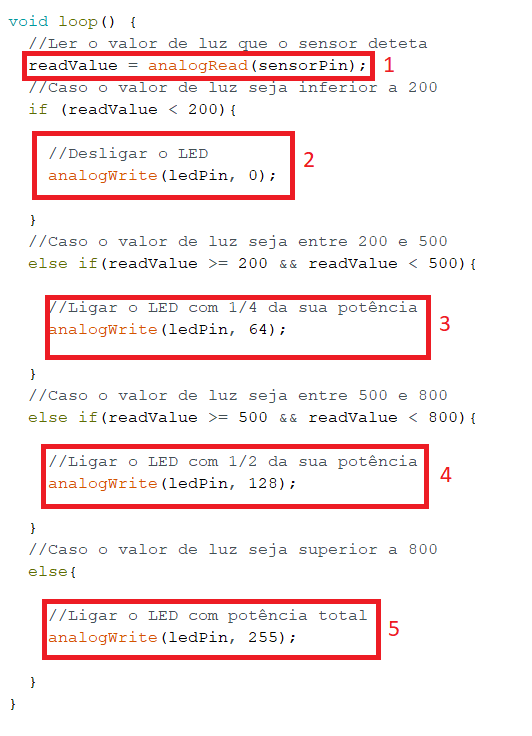
\includegraphics[scale=0.5]{images/codigo/sisA_ledvalues.png}
    \selectlanguage{portuguese}\caption{Código para os níveis o LED}
\end{figure}


\begin{itemize}
    \item 1 - O valor do Fotorresistor é lido através da função analogRead no pino onde está ligado o mesmo.
    \item 2,3,4,5 - Para o caso do LED estar compreendido dentro dos valores do "if", o mesmo é acendido com diferentes valores de potência. 
\end{itemize}

\begin{figure}[H]
    \centering
    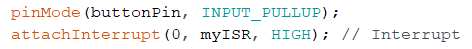
\includegraphics[scale=0.5]{images/codigo/sisA_interruptsetup.png}
    \selectlanguage{portuguese}\caption{Código para o setup do interrupt}
\end{figure}

\begin{figure}[H]
    \centering
    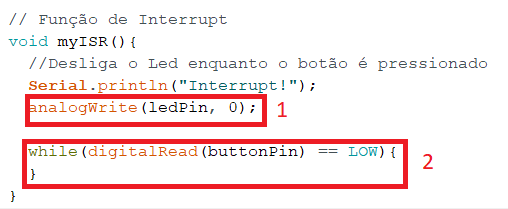
\includegraphics[scale=0.5]{images/codigo/sisA_interruptfunction.png}
    \selectlanguage{portuguese}\caption{Código para a função do interrupt}
\end{figure}

\begin{itemize}
    \item 1 - O LED é desligado durante o interrupt.
    \item 2 - Enquanto o botão se encontra pressionado, este "while" mantém a função de interrupt a correr.
\end{itemize}
